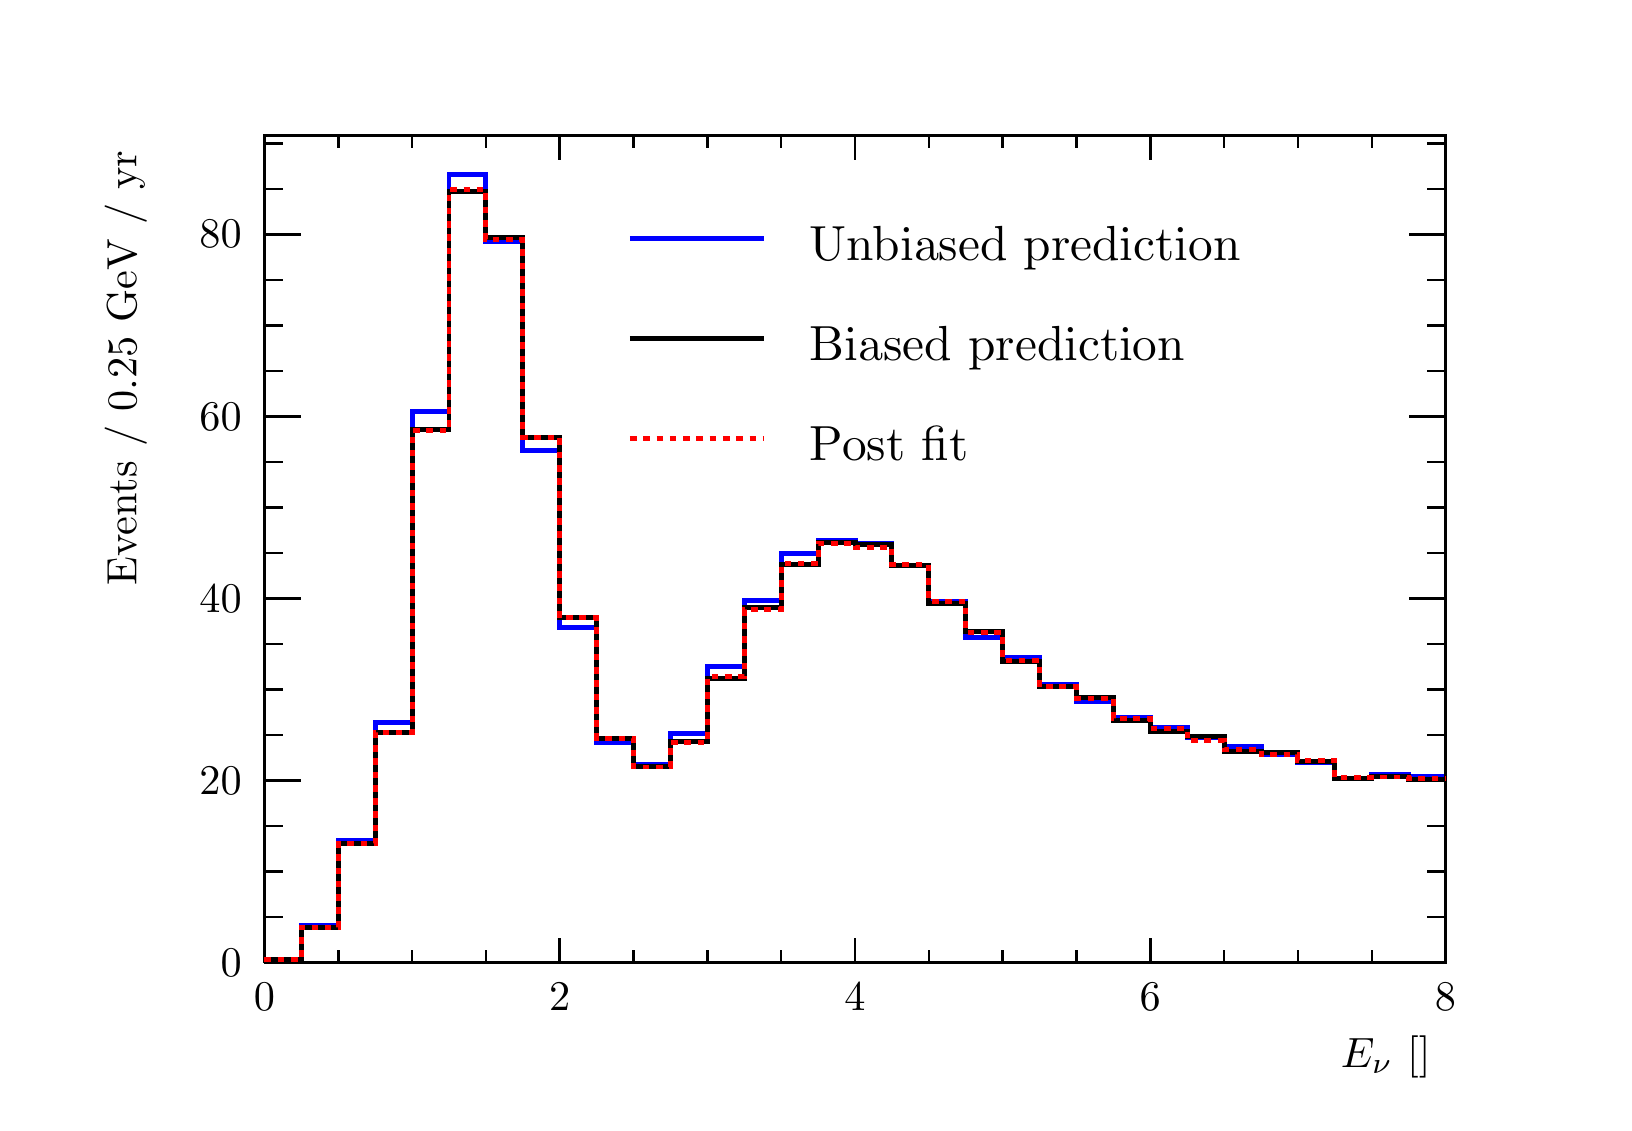
\begin{tikzpicture}
\pgfdeclareplotmark{cross} {
\pgfpathmoveto{\pgfpoint{-0.3\pgfplotmarksize}{\pgfplotmarksize}}
\pgfpathlineto{\pgfpoint{+0.3\pgfplotmarksize}{\pgfplotmarksize}}
\pgfpathlineto{\pgfpoint{+0.3\pgfplotmarksize}{0.3\pgfplotmarksize}}
\pgfpathlineto{\pgfpoint{+1\pgfplotmarksize}{0.3\pgfplotmarksize}}
\pgfpathlineto{\pgfpoint{+1\pgfplotmarksize}{-0.3\pgfplotmarksize}}
\pgfpathlineto{\pgfpoint{+0.3\pgfplotmarksize}{-0.3\pgfplotmarksize}}
\pgfpathlineto{\pgfpoint{+0.3\pgfplotmarksize}{-1.\pgfplotmarksize}}
\pgfpathlineto{\pgfpoint{-0.3\pgfplotmarksize}{-1.\pgfplotmarksize}}
\pgfpathlineto{\pgfpoint{-0.3\pgfplotmarksize}{-0.3\pgfplotmarksize}}
\pgfpathlineto{\pgfpoint{-1.\pgfplotmarksize}{-0.3\pgfplotmarksize}}
\pgfpathlineto{\pgfpoint{-1.\pgfplotmarksize}{0.3\pgfplotmarksize}}
\pgfpathlineto{\pgfpoint{-0.3\pgfplotmarksize}{0.3\pgfplotmarksize}}
\pgfpathclose
\pgfusepathqstroke
}
\pgfdeclareplotmark{cross*} {
\pgfpathmoveto{\pgfpoint{-0.3\pgfplotmarksize}{\pgfplotmarksize}}
\pgfpathlineto{\pgfpoint{+0.3\pgfplotmarksize}{\pgfplotmarksize}}
\pgfpathlineto{\pgfpoint{+0.3\pgfplotmarksize}{0.3\pgfplotmarksize}}
\pgfpathlineto{\pgfpoint{+1\pgfplotmarksize}{0.3\pgfplotmarksize}}
\pgfpathlineto{\pgfpoint{+1\pgfplotmarksize}{-0.3\pgfplotmarksize}}
\pgfpathlineto{\pgfpoint{+0.3\pgfplotmarksize}{-0.3\pgfplotmarksize}}
\pgfpathlineto{\pgfpoint{+0.3\pgfplotmarksize}{-1.\pgfplotmarksize}}
\pgfpathlineto{\pgfpoint{-0.3\pgfplotmarksize}{-1.\pgfplotmarksize}}
\pgfpathlineto{\pgfpoint{-0.3\pgfplotmarksize}{-0.3\pgfplotmarksize}}
\pgfpathlineto{\pgfpoint{-1.\pgfplotmarksize}{-0.3\pgfplotmarksize}}
\pgfpathlineto{\pgfpoint{-1.\pgfplotmarksize}{0.3\pgfplotmarksize}}
\pgfpathlineto{\pgfpoint{-0.3\pgfplotmarksize}{0.3\pgfplotmarksize}}
\pgfpathclose
\pgfusepathqfillstroke
}
\pgfdeclareplotmark{newstar} {
\pgfpathmoveto{\pgfqpoint{0pt}{\pgfplotmarksize}}
\pgfpathlineto{\pgfqpointpolar{44}{0.5\pgfplotmarksize}}
\pgfpathlineto{\pgfqpointpolar{18}{\pgfplotmarksize}}
\pgfpathlineto{\pgfqpointpolar{-20}{0.5\pgfplotmarksize}}
\pgfpathlineto{\pgfqpointpolar{-54}{\pgfplotmarksize}}
\pgfpathlineto{\pgfqpointpolar{-90}{0.5\pgfplotmarksize}}
\pgfpathlineto{\pgfqpointpolar{234}{\pgfplotmarksize}}
\pgfpathlineto{\pgfqpointpolar{198}{0.5\pgfplotmarksize}}
\pgfpathlineto{\pgfqpointpolar{162}{\pgfplotmarksize}}
\pgfpathlineto{\pgfqpointpolar{134}{0.5\pgfplotmarksize}}
\pgfpathclose
\pgfusepathqstroke
}
\pgfdeclareplotmark{newstar*} {
\pgfpathmoveto{\pgfqpoint{0pt}{\pgfplotmarksize}}
\pgfpathlineto{\pgfqpointpolar{44}{0.5\pgfplotmarksize}}
\pgfpathlineto{\pgfqpointpolar{18}{\pgfplotmarksize}}
\pgfpathlineto{\pgfqpointpolar{-20}{0.5\pgfplotmarksize}}
\pgfpathlineto{\pgfqpointpolar{-54}{\pgfplotmarksize}}
\pgfpathlineto{\pgfqpointpolar{-90}{0.5\pgfplotmarksize}}
\pgfpathlineto{\pgfqpointpolar{234}{\pgfplotmarksize}}
\pgfpathlineto{\pgfqpointpolar{198}{0.5\pgfplotmarksize}}
\pgfpathlineto{\pgfqpointpolar{162}{\pgfplotmarksize}}
\pgfpathlineto{\pgfqpointpolar{134}{0.5\pgfplotmarksize}}
\pgfpathclose
\pgfusepathqfillstroke
}
\definecolor{c}{rgb}{1,1,1};
\draw [color=c, fill=c] (0,0) rectangle (20,13.639);
\draw [color=c, fill=c] (3,1.77307) rectangle (18,12.2751);
\definecolor{c}{rgb}{0,0,0};
\draw [c,line width=0.9] (3,1.77307) -- (3,12.2751) -- (18,12.2751) -- (18,1.77307) -- (3,1.77307);
\definecolor{c}{rgb}{1,1,1};
\draw [color=c, fill=c] (3,1.77307) rectangle (18,12.2751);
\definecolor{c}{rgb}{0,0,0};
\draw [c,line width=0.9] (3,1.77307) -- (3,12.2751) -- (18,12.2751) -- (18,1.77307) -- (3,1.77307);
\definecolor{c}{rgb}{0,0,1};
\draw [c,line width=1.8] (3,1.80845) -- (3.46875,1.80845) -- (3.46875,2.24371) -- (3.9375,2.24371) -- (3.9375,3.32676) -- (4.40625,3.32676) -- (4.40625,4.8231) -- (4.875,4.8231) -- (4.875,8.77637) -- (5.34375,8.77637) -- (5.34375,11.775) --
 (5.8125,11.775) -- (5.8125,10.9239) -- (6.28125,10.9239) -- (6.28125,8.27142) -- (6.75,8.27142) -- (6.75,6.0318) -- (7.21875,6.0318) -- (7.21875,4.5663) -- (7.6875,4.5663) -- (7.6875,4.28576) -- (8.15625,4.28576) -- (8.15625,4.67989) --
 (8.625,4.67989) -- (8.625,5.53405) -- (9.09375,5.53405) -- (9.09375,6.37223) -- (9.5625,6.37223) -- (9.5625,6.96814) -- (10.0312,6.96814) -- (10.0312,7.13108) -- (10.5,7.13108) -- (10.5,7.08996) -- (10.9688,7.08996) -- (10.9688,6.80973) --
 (11.4375,6.80973) -- (11.4375,6.35593) -- (11.9062,6.35593) -- (11.9062,5.9002) -- (12.375,5.9002) -- (12.375,5.65128) -- (12.8438,5.65128) -- (12.8438,5.30575) -- (13.3125,5.30575) -- (13.3125,5.0826) -- (13.7812,5.0826) -- (13.7812,4.88684) --
 (14.25,4.88684) -- (14.25,4.75237) -- (14.7188,4.75237) -- (14.7188,4.62832) -- (15.1875,4.62832) -- (15.1875,4.51751) -- (15.6562,4.51751) -- (15.6562,4.41544) -- (16.125,4.41544) -- (16.125,4.31859) -- (16.5938,4.31859) -- (16.5938,4.11271) --
 (17.0625,4.11271) -- (17.0625,4.15666) -- (17.5312,4.15666) -- (17.5312,4.13901) -- (18,4.13901);
\definecolor{c}{rgb}{0,0,0};
\draw [c,line width=0.9] (3,1.77307) -- (18,1.77307);
\draw [c,line width=0.9] (3,2.07994) -- (3,1.77307);
\draw [c,line width=0.9] (3.9375,1.9265) -- (3.9375,1.77307);
\draw [c,line width=0.9] (4.875,1.9265) -- (4.875,1.77307);
\draw [c,line width=0.9] (5.8125,1.9265) -- (5.8125,1.77307);
\draw [c,line width=0.9] (6.75,2.07994) -- (6.75,1.77307);
\draw [c,line width=0.9] (7.6875,1.9265) -- (7.6875,1.77307);
\draw [c,line width=0.9] (8.625,1.9265) -- (8.625,1.77307);
\draw [c,line width=0.9] (9.5625,1.9265) -- (9.5625,1.77307);
\draw [c,line width=0.9] (10.5,2.07994) -- (10.5,1.77307);
\draw [c,line width=0.9] (11.4375,1.9265) -- (11.4375,1.77307);
\draw [c,line width=0.9] (12.375,1.9265) -- (12.375,1.77307);
\draw [c,line width=0.9] (13.3125,1.9265) -- (13.3125,1.77307);
\draw [c,line width=0.9] (14.25,2.07994) -- (14.25,1.77307);
\draw [c,line width=0.9] (15.1875,1.9265) -- (15.1875,1.77307);
\draw [c,line width=0.9] (16.125,1.9265) -- (16.125,1.77307);
\draw [c,line width=0.9] (17.0625,1.9265) -- (17.0625,1.77307);
\draw [c,line width=0.9] (18,2.07994) -- (18,1.77307);
\draw [anchor=base] (3,1.15931) node[scale=1.52731, color=c, rotate=0]{0};
\draw [anchor=base] (6.75,1.15931) node[scale=1.52731, color=c, rotate=0]{2};
\draw [anchor=base] (10.5,1.15931) node[scale=1.52731, color=c, rotate=0]{4};
\draw [anchor=base] (14.25,1.15931) node[scale=1.52731, color=c, rotate=0]{6};
\draw [anchor=base] (18,1.15931) node[scale=1.52731, color=c, rotate=0]{8};
\draw [anchor= east] (18,0.572837) node[scale=1.52731, color=c, rotate=0]{$E_{\nu}$ [\si{\GeV}]};
\draw [c,line width=0.9] (3,12.2751) -- (18,12.2751);
\draw [c,line width=0.9] (3,11.9682) -- (3,12.2751);
\draw [c,line width=0.9] (3.9375,12.1216) -- (3.9375,12.2751);
\draw [c,line width=0.9] (4.875,12.1216) -- (4.875,12.2751);
\draw [c,line width=0.9] (5.8125,12.1216) -- (5.8125,12.2751);
\draw [c,line width=0.9] (6.75,11.9682) -- (6.75,12.2751);
\draw [c,line width=0.9] (7.6875,12.1216) -- (7.6875,12.2751);
\draw [c,line width=0.9] (8.625,12.1216) -- (8.625,12.2751);
\draw [c,line width=0.9] (9.5625,12.1216) -- (9.5625,12.2751);
\draw [c,line width=0.9] (10.5,11.9682) -- (10.5,12.2751);
\draw [c,line width=0.9] (11.4375,12.1216) -- (11.4375,12.2751);
\draw [c,line width=0.9] (12.375,12.1216) -- (12.375,12.2751);
\draw [c,line width=0.9] (13.3125,12.1216) -- (13.3125,12.2751);
\draw [c,line width=0.9] (14.25,11.9682) -- (14.25,12.2751);
\draw [c,line width=0.9] (15.1875,12.1216) -- (15.1875,12.2751);
\draw [c,line width=0.9] (16.125,12.1216) -- (16.125,12.2751);
\draw [c,line width=0.9] (17.0625,12.1216) -- (17.0625,12.2751);
\draw [c,line width=0.9] (18,11.9682) -- (18,12.2751);
\draw [c,line width=0.9] (3,1.77307) -- (3,12.2751);
\draw [c,line width=0.9] (3.462,1.77307) -- (3,1.77307);
\draw [c,line width=0.9] (3.231,2.35107) -- (3,2.35107);
\draw [c,line width=0.9] (3.231,2.92908) -- (3,2.92908);
\draw [c,line width=0.9] (3.231,3.50709) -- (3,3.50709);
\draw [c,line width=0.9] (3.462,4.08509) -- (3,4.08509);
\draw [c,line width=0.9] (3.231,4.6631) -- (3,4.6631);
\draw [c,line width=0.9] (3.231,5.24111) -- (3,5.24111);
\draw [c,line width=0.9] (3.231,5.81912) -- (3,5.81912);
\draw [c,line width=0.9] (3.462,6.39712) -- (3,6.39712);
\draw [c,line width=0.9] (3.231,6.97513) -- (3,6.97513);
\draw [c,line width=0.9] (3.231,7.55314) -- (3,7.55314);
\draw [c,line width=0.9] (3.231,8.13114) -- (3,8.13114);
\draw [c,line width=0.9] (3.462,8.70915) -- (3,8.70915);
\draw [c,line width=0.9] (3.231,9.28716) -- (3,9.28716);
\draw [c,line width=0.9] (3.231,9.86516) -- (3,9.86516);
\draw [c,line width=0.9] (3.231,10.4432) -- (3,10.4432);
\draw [c,line width=0.9] (3.462,11.0212) -- (3,11.0212);
\draw [c,line width=0.9] (3.462,11.0212) -- (3,11.0212);
\draw [c,line width=0.9] (3.231,11.5992) -- (3,11.5992);
\draw [c,line width=0.9] (3.231,12.1772) -- (3,12.1772);
\draw [anchor= east] (2.9,1.77307) node[scale=1.52731, color=c, rotate=0]{0};
\draw [anchor= east] (2.9,4.08509) node[scale=1.52731, color=c, rotate=0]{20};
\draw [anchor= east] (2.9,6.39712) node[scale=1.52731, color=c, rotate=0]{40};
\draw [anchor= east] (2.9,8.70915) node[scale=1.52731, color=c, rotate=0]{60};
\draw [anchor= east] (2.9,11.0212) node[scale=1.52731, color=c, rotate=0]{80};
\draw [anchor= east] (1.24,12.2751) node[scale=1.52731, color=c, rotate=90]{Events / 0.25 GeV / yr};
\draw [c,line width=0.9] (18,1.77307) -- (18,12.2751);
\draw [c,line width=0.9] (17.538,1.77307) -- (18,1.77307);
\draw [c,line width=0.9] (17.769,2.35107) -- (18,2.35107);
\draw [c,line width=0.9] (17.769,2.92908) -- (18,2.92908);
\draw [c,line width=0.9] (17.769,3.50709) -- (18,3.50709);
\draw [c,line width=0.9] (17.538,4.08509) -- (18,4.08509);
\draw [c,line width=0.9] (17.769,4.6631) -- (18,4.6631);
\draw [c,line width=0.9] (17.769,5.24111) -- (18,5.24111);
\draw [c,line width=0.9] (17.769,5.81912) -- (18,5.81912);
\draw [c,line width=0.9] (17.538,6.39712) -- (18,6.39712);
\draw [c,line width=0.9] (17.769,6.97513) -- (18,6.97513);
\draw [c,line width=0.9] (17.769,7.55314) -- (18,7.55314);
\draw [c,line width=0.9] (17.769,8.13114) -- (18,8.13114);
\draw [c,line width=0.9] (17.538,8.70915) -- (18,8.70915);
\draw [c,line width=0.9] (17.769,9.28716) -- (18,9.28716);
\draw [c,line width=0.9] (17.769,9.86516) -- (18,9.86516);
\draw [c,line width=0.9] (17.769,10.4432) -- (18,10.4432);
\draw [c,line width=0.9] (17.538,11.0212) -- (18,11.0212);
\draw [c,line width=0.9] (17.538,11.0212) -- (18,11.0212);
\draw [c,line width=0.9] (17.769,11.5992) -- (18,11.5992);
\draw [c,line width=0.9] (17.769,12.1772) -- (18,12.1772);
\draw [c,line width=1.8] (3,1.80845) -- (3.46875,1.80845) -- (3.46875,2.22212) -- (3.9375,2.22212) -- (3.9375,3.28005) -- (4.40625,3.28005) -- (4.40625,4.69844) -- (4.875,4.69844) -- (4.875,8.53883) -- (5.34375,8.53883) -- (5.34375,11.5639) --
 (5.8125,11.5639) -- (5.8125,10.982) -- (6.28125,10.982) -- (6.28125,8.43741) -- (6.75,8.43741) -- (6.75,6.15267) -- (7.21875,6.15267) -- (7.21875,4.61781) -- (7.6875,4.61781) -- (7.6875,4.25773) -- (8.15625,4.25773) -- (8.15625,4.57876) --
 (8.625,4.57876) -- (8.625,5.3828) -- (9.09375,5.3828) -- (9.09375,6.28229) -- (9.5625,6.28229) -- (9.5625,6.83044) -- (10.0312,6.83044) -- (10.0312,7.11077) -- (10.5,7.11077) -- (10.5,7.08248) -- (10.9688,7.08248) -- (10.9688,6.81056) --
 (11.4375,6.81056) -- (11.4375,6.338) -- (11.9062,6.338) -- (11.9062,5.97956) -- (12.375,5.97956) -- (12.375,5.59531) -- (12.8438,5.59531) -- (12.8438,5.28172) -- (13.3125,5.28172) -- (13.3125,5.13482) -- (13.7812,5.13482) -- (13.7812,4.85327) --
 (14.25,4.85327) -- (14.25,4.70569) -- (14.7188,4.70569) -- (14.7188,4.64086) -- (15.1875,4.64086) -- (15.1875,4.45932) -- (15.6562,4.45932) -- (15.6562,4.44126) -- (16.125,4.44126) -- (16.125,4.32169) -- (16.5938,4.32169) -- (16.5938,4.11582) --
 (17.0625,4.11582) -- (17.0625,4.13147) -- (17.5312,4.13147) -- (17.5312,4.09626) -- (18,4.09626);
\definecolor{c}{rgb}{1,0,0};
\draw [c,dash pattern=on 2.40pt off 2.40pt ,line width=1.8] (3,1.80889) -- (3.46875,1.80889) -- (3.46875,2.22302) -- (3.9375,2.22302) -- (3.9375,3.28572) -- (4.40625,3.28572) -- (4.40625,4.69548) -- (4.875,4.69548) -- (4.875,8.52609) --
 (5.34375,8.52609) -- (5.34375,11.5956) -- (5.8125,11.5956) -- (5.8125,10.9533) -- (6.28125,10.9533) -- (6.28125,8.44458) -- (6.75,8.44458) -- (6.75,6.15122) -- (7.21875,6.15122) -- (7.21875,4.62287) -- (7.6875,4.62287) -- (7.6875,4.25652) --
 (8.15625,4.25652) -- (8.15625,4.57099) -- (8.625,4.57099) -- (8.625,5.4072) -- (9.09375,5.4072) -- (9.09375,6.25725) -- (9.5625,6.25725) -- (9.5625,6.84247) -- (10.0312,6.84247) -- (10.0312,7.09794) -- (10.5,7.09794) -- (10.5,7.05015) --
 (10.9688,7.05015) -- (10.9688,6.82594) -- (11.4375,6.82594) -- (11.4375,6.35998) -- (11.9062,6.35998) -- (11.9062,5.96743) -- (12.375,5.96743) -- (12.375,5.60458) -- (12.8438,5.60458) -- (12.8438,5.27536) -- (13.3125,5.27536) -- (13.3125,5.1302) --
 (13.7812,5.1302) -- (13.7812,4.8667) -- (14.25,4.8667) -- (14.25,4.74938) -- (14.7188,4.74938) -- (14.7188,4.58762) -- (15.1875,4.58762) -- (15.1875,4.47806) -- (15.6562,4.47806) -- (15.6562,4.41311) -- (16.125,4.41311) -- (16.125,4.34178) --
 (16.5938,4.34178) -- (16.5938,4.12595) -- (17.0625,4.12595) -- (17.0625,4.12942) -- (17.5312,4.12942) -- (17.5312,4.10746) -- (18,4.10746);
\definecolor{c}{rgb}{1,1,1};
\draw [color=c, fill=c] (7.27794,7.7937) rectangle (16.9914,11.6046);
\definecolor{c}{rgb}{0,0,0};
\draw [anchor=base west] (9.7063,10.6836) node[scale=1.78187, color=c, rotate=0]{Unbiased prediction};
\definecolor{c}{rgb}{0,0,1};
\draw [c,line width=1.8] (7.64219,10.9694) -- (9.34205,10.9694);
\definecolor{c}{rgb}{0,0,0};
\draw [anchor=base west] (9.7063,9.41332) node[scale=1.78187, color=c, rotate=0]{Biased prediction};
\draw [c,line width=1.8] (7.64219,9.69914) -- (9.34205,9.69914);
\draw [anchor=base west] (9.7063,8.14303) node[scale=1.78187, color=c, rotate=0]{Post fit};
\definecolor{c}{rgb}{1,0,0};
\draw [c,dash pattern=on 2.40pt off 2.40pt ,line width=1.8] (7.64219,8.42884) -- (9.34205,8.42884);
\end{tikzpicture}
